\documentclass[../main.tex]{subfiles}
\graphicspath{
    {"../img/"}
    {"img/"}
}

\begin{document}
    \subsection{Równanie ciągłości}
    Mamy rurę między punktami $a$, i $b$ i przechodzą przez nią biedronki. Przez $A(t)$ oznaczamy całkowitą liczbę biedronek w rurze. $U(x,t)$ to liczba biedronek w punkcie $x$ w czasie $t$.
    \begin{equation}
        \label{eqn:w2-1}
        A(t) = \int\limits_{a}^{b} U(x,t)dx
    \end{equation}

I na przykład mamy tak
\begin{enumerate}
    \item $t = 1 \implies A(1) = 7$
    \item $t = 2 \implies A(2) = 9$
    \item $t = 3 \implies A(3) = 15$
    \item \ldots
    \item $t = 7 \implies A(7) = 349$
\end{enumerate}
Na przykład możemy sobie zadać pytanie ile to jest $A(3) - A(2)$?\\
No my wiemy, to jest $A(3) - A(2) = 15 - 9$. Ale za to można to napisać tak:
\[
    A(3) - A(2) = \phi(a, \_) - \phi(b, \_) + \int\limits_{a}^{b} f(x, \_)dx
.\]
Tam $\phi$ to ruch na brzegach, a $f$ to ile biedronek się zmęczyło w rurze.\\
To teraz wersja v2.0. Co będzie dla  $t, t+\Delta t$?
 \[
     A(t+\Delta t) - A(t) = \int\limits_{t}^{t + \Delta t} \left( \phi\left(a, \xi\right) - \phi\left(b, \xi\right) \right)  d\xi + \int\limits_{t}^{t+\Delta t} \int\limits_{a}^{b} f(x,\xi)dxd\xi
.\]
Dzielimy przez $\Delta t$ i przechodzimy z granicą do zera.
\[
    \frac{\partial A}{\partial t} = \phi(a,t) - \phi(b,t) + \int\limits_{a}^{b} f(x,t)dx
.\]
Wiemy jak wygląda \eqref{eqn:w2-1}
\[
    \int\limits_{a}^{b} \frac{\partial U}{\partial t} dx = -\int\limits_{a}^{b} \frac{\partial \phi}{\partial x} dx + \int\limits_{a}^{b} f(x,t)dx
.\]
Teraz strzelamy w wyrażenie podcałkowe
\[
    \frac{\partial U}{\partial t} + \frac{\partial \phi}{\partial x} = f(x,t)
.\]
I to jest równanie ciągłości. Do modelu przechodzenia biedronek przez rurę możemy wkładać funkcje $\phi$. Na razie wiemy tylko coś tam o przepływie (coś wchodzi, wychodzi albo nie).
\begin{pytanie}|
    \begin{enumerate}
        \item Czy $\phi$ może zadać nam dynamikę w tej rurze?
        \item Jak mamy dobrać te $\phi$?
    \end{enumerate}
\end{pytanie}
\begin{enumerate}
    \item Załóżmy na początek, że $\phi \sim U$, czyli np. adwekcja
\[
    \phi = c \cdot U,\quad f = 0
.\]
\[
    \frac{\partial U}{\partial t} + (c \cdot U)_{,x} = 0
.\]
Ale jak my mamy takie równanie różniczkowe
\[
    \frac{\partial U(x,t)}{\partial t} + c \frac{\partial U(x,t)}{\partial x} = 0
.\]
Ważne jest, żeby z takiego równania wyciągnąć sobie metodologię, która do niego doprowadziła - to może pomóc w szukaniu rozwiązań.\\
    \item Weźmy na przykład
\[
    U(x,t) = F(x - ct)
,\]
gdzie $F\in \mathcal{C}^1(\mathbb{R})$. Jak podstawimy, to mamy
\[
    \frac{\partial }{\partial t} F(x-ct) + c \frac{\partial F(x-ct)}{\partial x} = F'(c) + c \cdot F' = 0
.\]
Czyli to równanie spełnia dowolna funkcja, która przesuwa się w którąś stronę (prawo albo lewo). Na przykład taka hałda mrówek idąca przez rurę, albo maszerująca kolumna wojska.

\item Inny przypadek:
\[
    \phi = c \cdot U_{,x}
.\]
Teraz dostaniemy takie równanie
\[
    \frac{\partial U}{\partial t} + c \cdot U_{,x x} =0
,\]
czyli równanie dyfuzji, (przepływ ciepła przez długi pręt albo równanie Schrödingera).

\item Jeszcze inny przypadek
\[
    \phi = c \cdot U_{,x} + d \cdot U
.\]
I teraz wychodzi
\[
    \frac{\partial U}{\partial t} + c \cdot U_{,xx} + d \cdot U_{,x} = 0
.\]

\item Można włożyć własności pręta
\[
    \phi = k(U) \cdot U_{,x}
.\]
\item Ciecz radioaktywna (wlewamy coś do rury, ale nam to po drodze trochę znika)\\
    Rozpad radioaktywny to było coś takiego
        \[
            \frac{\partial U}{\partial t} = -\lambda U
        .\]
    No to może
        \[
            \frac{\partial U}{\partial t} + c \cdot U_{,x} = -\lambda U
        .\]
    A rozwój bakterii był taki:
        \[
            \frac{\partial U}{\partial t} = \lambda U
        .\]
    Jak powiązać tempo namnażania z jakąś graniczną wielkością? (taka nie-nieskończona skrzynka)\\
Rozwój z ograniczeniem
    \[
        \frac{\partial U}{\partial t} = U \cdot \left( 1 - \frac{U}{\kappa} \right)
    ,\]
a $\kappa$ to gęstość graniczna.
\item Ruch samochodów
    \[
        \frac{\partial U}{\partial t} + \phi(U) = 0
    .\]
$\phi$ bierzemy takie
\[
    \phi = \left(1 - \frac{U}{\kappa}\right) U
.\]
\[
    \frac{\partial U}{\partial t} + \left( \left( 1 - \frac{U}{\kappa} \right) U \right)_{,x} = 0
.\]
(KDW)
\item Jeszcze jest np. równanie Burgersa, ale ono to już nawet liniowe nie jest.
    \[
        \frac{\partial U}{\partial t} + \left( \frac{U^2}{2} \right) _{,x} = 0
.\]
\end{enumerate}
To jeszcze takie śmieszne $\phi$, które patrzy co się dzieje dookoła
\[
    \phi(x) = \frac{\phi(x-h) + \phi(x+h)}{2}
.\]

\subsection{Metoda charakterystyk}
Chcemy rozwiązać równanie
\begin{align}
    \label{eqn:w2-2}
    &\frac{\partial U(x,t)}{\partial t} + c\frac{\partial U(x,t)}{\partial x} = 0,\quad U:\mathbb{R}\times \left]0,\infty\right[\to \mathbb{R}\\
    &U(x,0) = U_0(x)\nonumber
\end{align}
\eqref{eqn:w2-2} możemy zapisać tak
\[
    \left[ U_{,t}, U_{x} \right] \begin{bmatrix} 1\\c \end{bmatrix} = 0
.\]
Wiemy, że gradient funkcji jest prostopadły do poziomicy. Oznacza to, że jeżeli $\left(x(s), t(s)\right)$ - krzywa taka, że
\[
    U(x(s), t(s)) = const,\quad s\in \mathbb{R}_+
.\]
$\left( x(s), t(s) \right) $ - parametryzacja poziomicy.

Wiemy, że wektor $\begin{bmatrix} 1\\c \end{bmatrix} $ musi być styczny do poziomicy, czyli
    \[
        \frac{\partial x}{\partial s} = c,\quad \frac{\partial t}{\partial s} = 1
    .\]
Stąd mamy
\[
    x = c \cdot s + x_0,\quad t = s+ t_0
.\]
Z drugiego bierzemy $s = t - t_0$ i wsadzamy do pierwszego i wychodzi
\[
    x = c(t-t_0) + x_0
.\]
Więc na każdej linii $U(x(s), t(s)) = const$, jak na rys \ref{fig:poziomice}
 \begin{figure}[h]
    \centering
    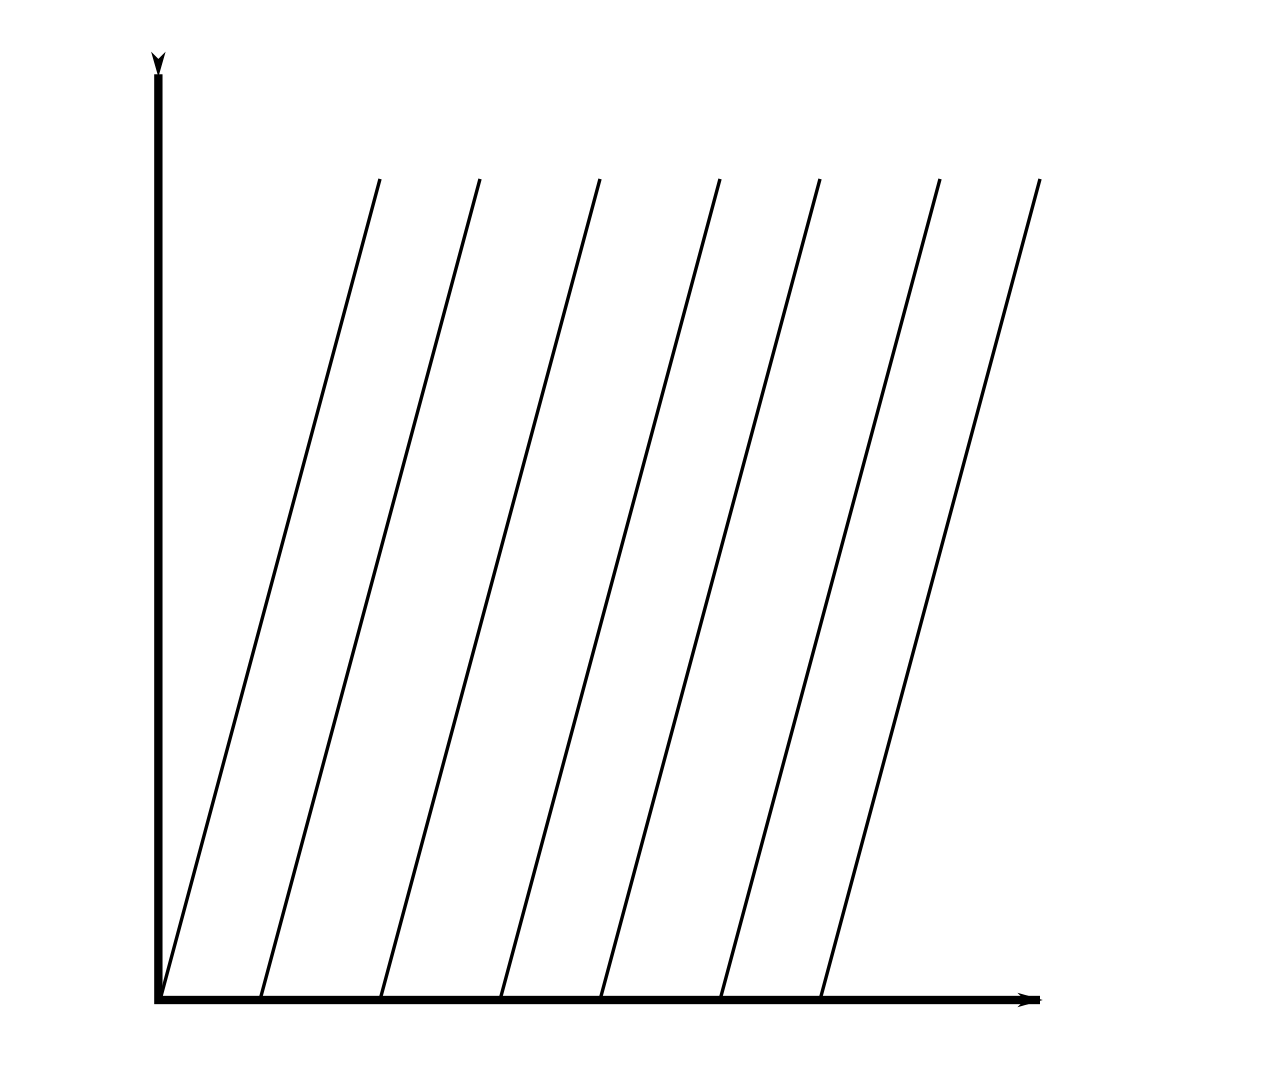
\includegraphics[width=0.2\textwidth]{poziomice}
    \caption{Fajne poziomice}
    \label{fig:poziomice}
\end{figure}

Skoro wiemy, że $U(x(s),t(s))$ jest stała, to
\begin{align*}
    \frac{d}{ds} U\left( x(s), t(s) \right) &= \frac{\partial U}{\partial x} \frac{\partial x}{\partial s} + \frac{\partial U}{\partial t} \frac{\partial t}{\partial s} = \\
    &= c \cdot \frac{\partial U}{\partial x} + \frac{\partial U}{\partial t} = 0
.\end{align*}
Zmieńmy parametryzację. Niech $s = t$, wówczas
\[
    U\left( c(t-t_0) + x_0, t \right) = const
.\]
\begin{pytanie}
Ile wynosi wartość na poziomicy?
\end{pytanie}
\textbf{Odpowiedź: } Dla krzywej $x = c(t-t_0) + x_0$, $U(x,t) = U_0(x_0)$, ale
\[
    x_0 = x - c(t-t_0)
.\]
No to trzeba wstawić
\[
    U(x,t) = U_0\left( x - c(t-t_0) \right)
.\]
\begin{pytanie}
    Gdzie się to psuje?
\end{pytanie}
\begin{figure}[h]
    \centering
    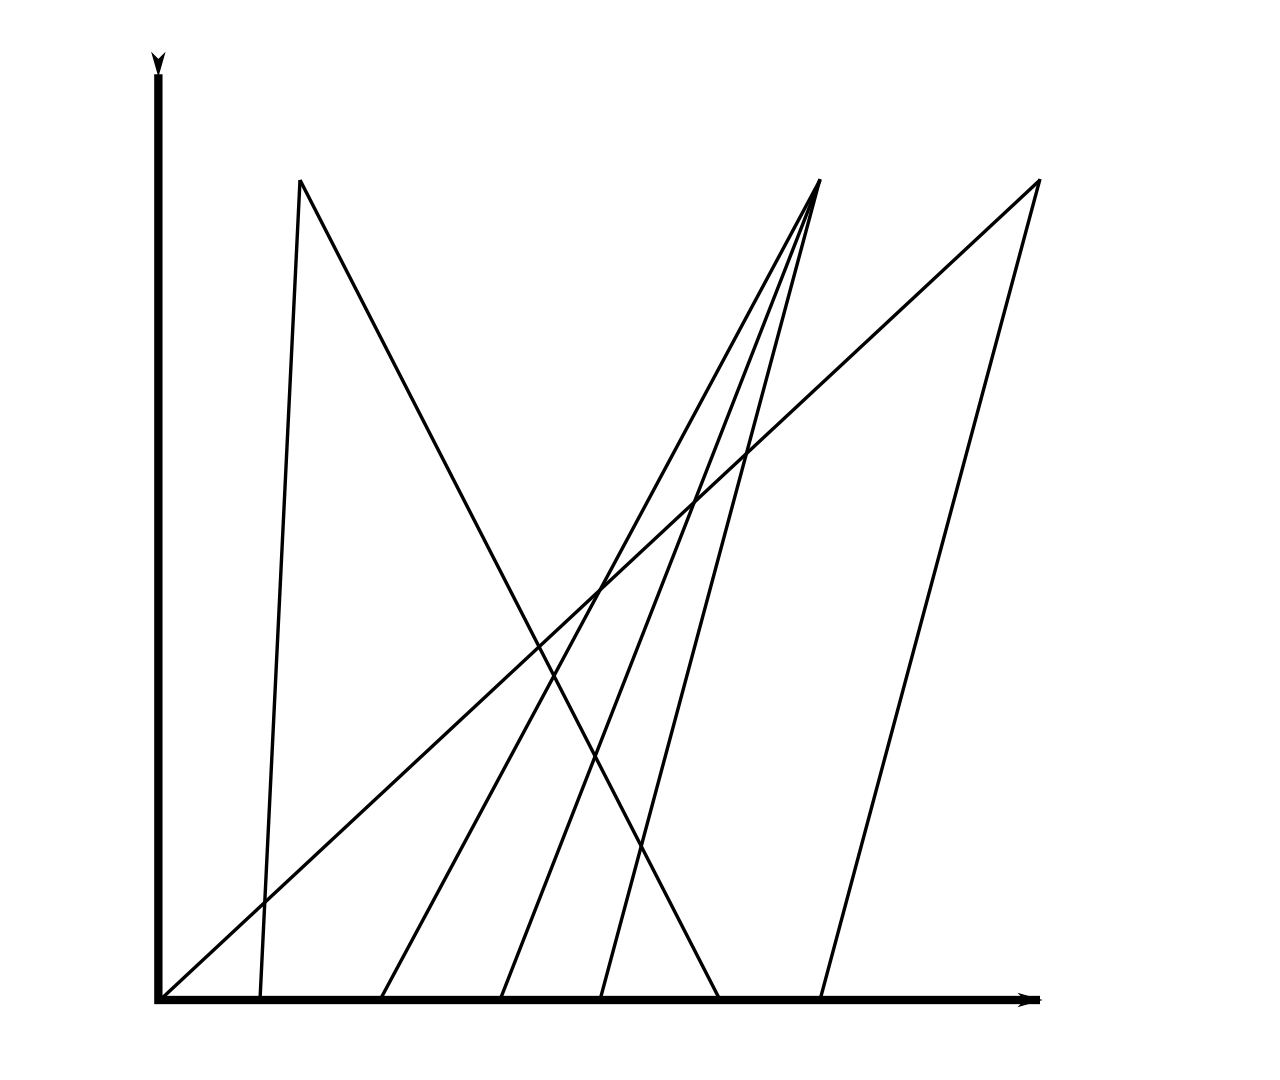
\includegraphics[width=0.2\textwidth]{zepsute-poziomice}
    \caption{Zepsute przecinające się poziomice}
    \label{fig:zepsute-poziomice}
\end{figure}
\textbf{Odpowiedź: } Problem się pojawia jak te poziomice zaczynają się przecinać. Bo co to wtedy znaczy, że funkcja jest stała na takiej poziomicy?


\begin{przyklad}
    (trochę o równaniu Burgersa)\\
    \[
        U_{,t} + U \cdot U_{,x} = 0
    .\]
Wygląda strasznie, ale jak zapiszemy tak
\[
    \left[ U_{,t}, U_{,x} \right] \begin{bmatrix} 1\\U \end{bmatrix} = 0
.\]
To się okazuje, że dostajemy równania na poziomice.
\[
    \frac{\partial x}{\partial s} = U\left( x(s), t(s) \right) ,\quad \frac{\partial t}{\partial s} = 1
.\]
\end{przyklad}

\end{document}
